% !TEX encoding = UTF-8
% !TEX TS-program = pdflatex
% !TEX root = ../tesi.tex
% !TEX spellcheck = it-IT

%**************************************************************
\chapter{Analisi dei Requisiti}
\label{cap:analisi-requisiti}
%**************************************************************

%\intro{Brevissima introduzione al capitolo}\\

%**************************************************************
\section{Descrizione di un generico sistema di sintesi vocale}
La \textbf{sintesi vocale} (in inglese \textit{speech synthesis}) è la tecnica per la riproduzione
artificiale della voce umana.\\ I sistemi di sintesi vocale (o sistemi \textbf{TTS}, dall'inglese \textit{Text To Speech})
 sono in genere composti da due parti interagenti ma operanti in ambiti differenti:
\begin{itemize}
  \item \textbf{front-end}: è la parte del sistema che si occupa della conversione del testo in \textit{input} in simboli fonetici 
                            interpretabili dal \textit{back-end};
  \item \textbf{back-end}: è la parte del sistema che interpreta e trasforma i simboli fonetici ricevuti in \textit{input} 
                           dal \textit{front-end}, producendo infine audio.
\end{itemize}
Il primo compito del \textit{front-end} è l'analisi del testo con lo scopo di espanderne i numeri, le sigle,
le date e le abbreviazioni in parole estese. \\
In una fase successiva le parole vengono convertite nelle trascrizioni fonetiche corrispondenti e viene
effettuata la suddivisione del testo in frasi e paragrafi. \\
I cinque processi del sistema nel suo complesso sono dunque:
\begin{itemize}
  \item \texttt{Tokenizer} (\textit{front-end}): processo che suddivide l'\textit{input} in \textit{utterance};
  \item \texttt{Espansione o normalizzazione} (\textit{front-end}): processo che espande o normalizza una \textit{utterance};
  \item \texttt{Phonemiser} (\textit{front-end}): processo che converte le parole nelle trascrizioni fonetiche corrispondenti;
  \item \texttt{Calcolo e raccolta delle feature} (\textit{front-end}): gruppo di processi che calcolano e aggiungono ulteriori
               informazioni alle \textit{utterance};
  \item \texttt{Vocoder} (\textit{back-end}): processo generatore dell'audio finale.
\end{itemize}

\begin{figure}[!h] 
    \centering 
    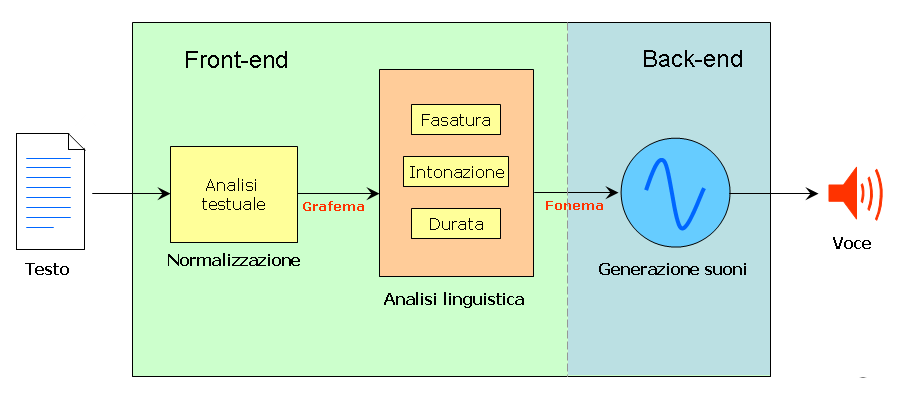
\includegraphics[width=0.9\columnwidth]{Sintesi_vocale} 
    \caption{Architettura di un sistema di \textbf{TTS}}
\end{figure}

\newpage

\section{Requisiti}
Di seguito viene riportata una lista esaustiva dei requisiti individuati all'inizio dell'attività di \textit{stage}.
Essi vengono classificati secondo i seguenti codici aggiunti in coda al carattere \textbf{R}:
%Da un'attenta analisi dei requisiti e degli use case effettuata sul progetto è stata stilata la tabella che traccia i requisiti in rapporto agli use case.\\
%Sono stati individuati diversi tipi di requisiti e si è quindi fatto utilizzo di un codice identificativo per distinguerli.\\
%Il codice dei requisiti è così strutturato R(F/Q/V)(N/D/O) dove:
\begin{enumerate}
    \item[\textbf{F} =] requisito funzionale;
    \item[\textbf{Q} =] requisito di qualità;
    \item[\textbf{V} =] requisito di vincolo;
    \item[\textbf{O} =] requisito obbligatorio;
    \item[\textbf{D} =] requisito desiderabile;
    \item[\textbf{Z} =] requisito opzionale.
\end{enumerate}
    %BEGIN of table
    %Tabella 
      \begin{center}
        \bgroup
        \def\arraystretch{1.8}
        \begin{longtable}{ | l | p{2cm} | p{4.7cm} | p{2.5cm} |}
        \hline
        \textbf{Requisito} & \textbf{Tipologia}
        & \textbf{Descrizione} \\ \hline
        RFO-1 & Funzionale \newline Obbligatorio & Implementazione di una voce sintetica in lingua italiana \newline  \\ \hline
        RFO-2 & Funzionale \newline Obbligatorio & Implementazione di un sillabificatore per la lingua italiana \newline  \\ \hline
        RQO-1 & Qualità \newline Obbligatorio & Implementazione di un'infrastruttura di \textit{test} per le componenti di 
                              trascrizione fonetica \newline  \\ \hline
        RFO-3 & Funzionale \newline Obbligatorio & Rappresentazione di tutte le informazioni
                              necessarie nelle \textit{label} (eventualmente con valori predefiniti) per il \textit{back-end} \newline  \\ \hline
         
        RFD-1 & Funzionale \newline Desiderabile & Integrazione di un sistema di dizionario efficace \newline  \\ \hline
        RQD-1 & Qualità \newline Desiderabile & Miglioramento del sistema di addestramento per
                        la componente \textit{letter-to-sound} \newline  \\ \hline
        RQD-2 & Qualità \newline Desiderabile & Implementazione di \textit{test} che permettano 
                il confronto con \textbf{MaryTTS} \newline  \\ \hline
        RQD-3 & Qualità \newline Desiderabile & Miglioramento del programma di esempio con cui si 
                interagisce con la libreria \textbf{Speect} \newline  \\ \hline                 

        RFZ-1 & Funzionale \newline Opzionale & Integrazione/Implementazione di nuove componenti 
                per la trascrizione fonetica \newline  \\ \hline

        \caption{Requisiti}
        \end{longtable}
        \egroup
     \end{center}
    %END of table
